\documentclass[a4paper, 11pt]{article}
\usepackage{graphicx}
\usepackage{amsmath}
\usepackage[pdftex]{hyperref}

% Lengths and indenting
\setlength{\textwidth}{16.5cm}
\setlength{\marginparwidth}{1.5cm}
\setlength{\parindent}{0cm}
\setlength{\parskip}{0.15cm}
\setlength{\textheight}{22cm}
\setlength{\oddsidemargin}{0cm}
\setlength{\evensidemargin}{\oddsidemargin}
\setlength{\topmargin}{0cm}
\setlength{\headheight}{0cm}
\setlength{\headsep}{0cm}

\renewcommand{\familydefault}{\sfdefault}

\title{Machine Learning 2015: Project 1 - Regression Report}
\author{jo@student.ethz.ch\\ sakhadov@student.ethz.ch\\ kevinlu@student.ethz.ch\\}
\date{\today}

\begin{document}
\maketitle

\section*{Experimental Protocol}
We used split-training (train on 80\%, test on 20\%) and cross-validation to select the best models.
Feature engineering on single columns did not yield good results.
Thus, the only transformation used was one hot encoding for `Width` and `Branches allowed`. In addition, log-transforming the y values yielded substantially better results.\\
We plotted single features to gain insight over their distribution and importance (see Section \ref{plots}).
The machine learning method \textit{random trees} reported several features as as very unimportant: L1 Dcache size, Branches allowed, L1 Icache size, L2 Ucache size.\\
In the end, we used Random Forest Regression, which yielded the best results and is very fast to train.

\section{Tools}
We used Python with the machine learning library \textit{scikit-learn} and \textit{numpy}.

\section{Algorithm}
\textit{Random forest regression} builds multiple decision trees during training (using randomization). Each tree makes a decision and the class with the most votes in the forest is chosen.

\section{Features}
We did not construct any new features, as it did not improve the performance in the settings we chose.

\section{Parameters}
Model validation was performed via cross-validation. We trained on 80\% of the data and tested with 20\%.

\section{Lessons Learned} In an alternative approach, we tested an \textit{artificial neural network} (ANN). However, it did not perform better than the \textit{random forest regressor}. Neural networks may be better suited when the explicit knowledge about the problem is very limited, for instance face recognition.

\section{Plots}\label{plots}
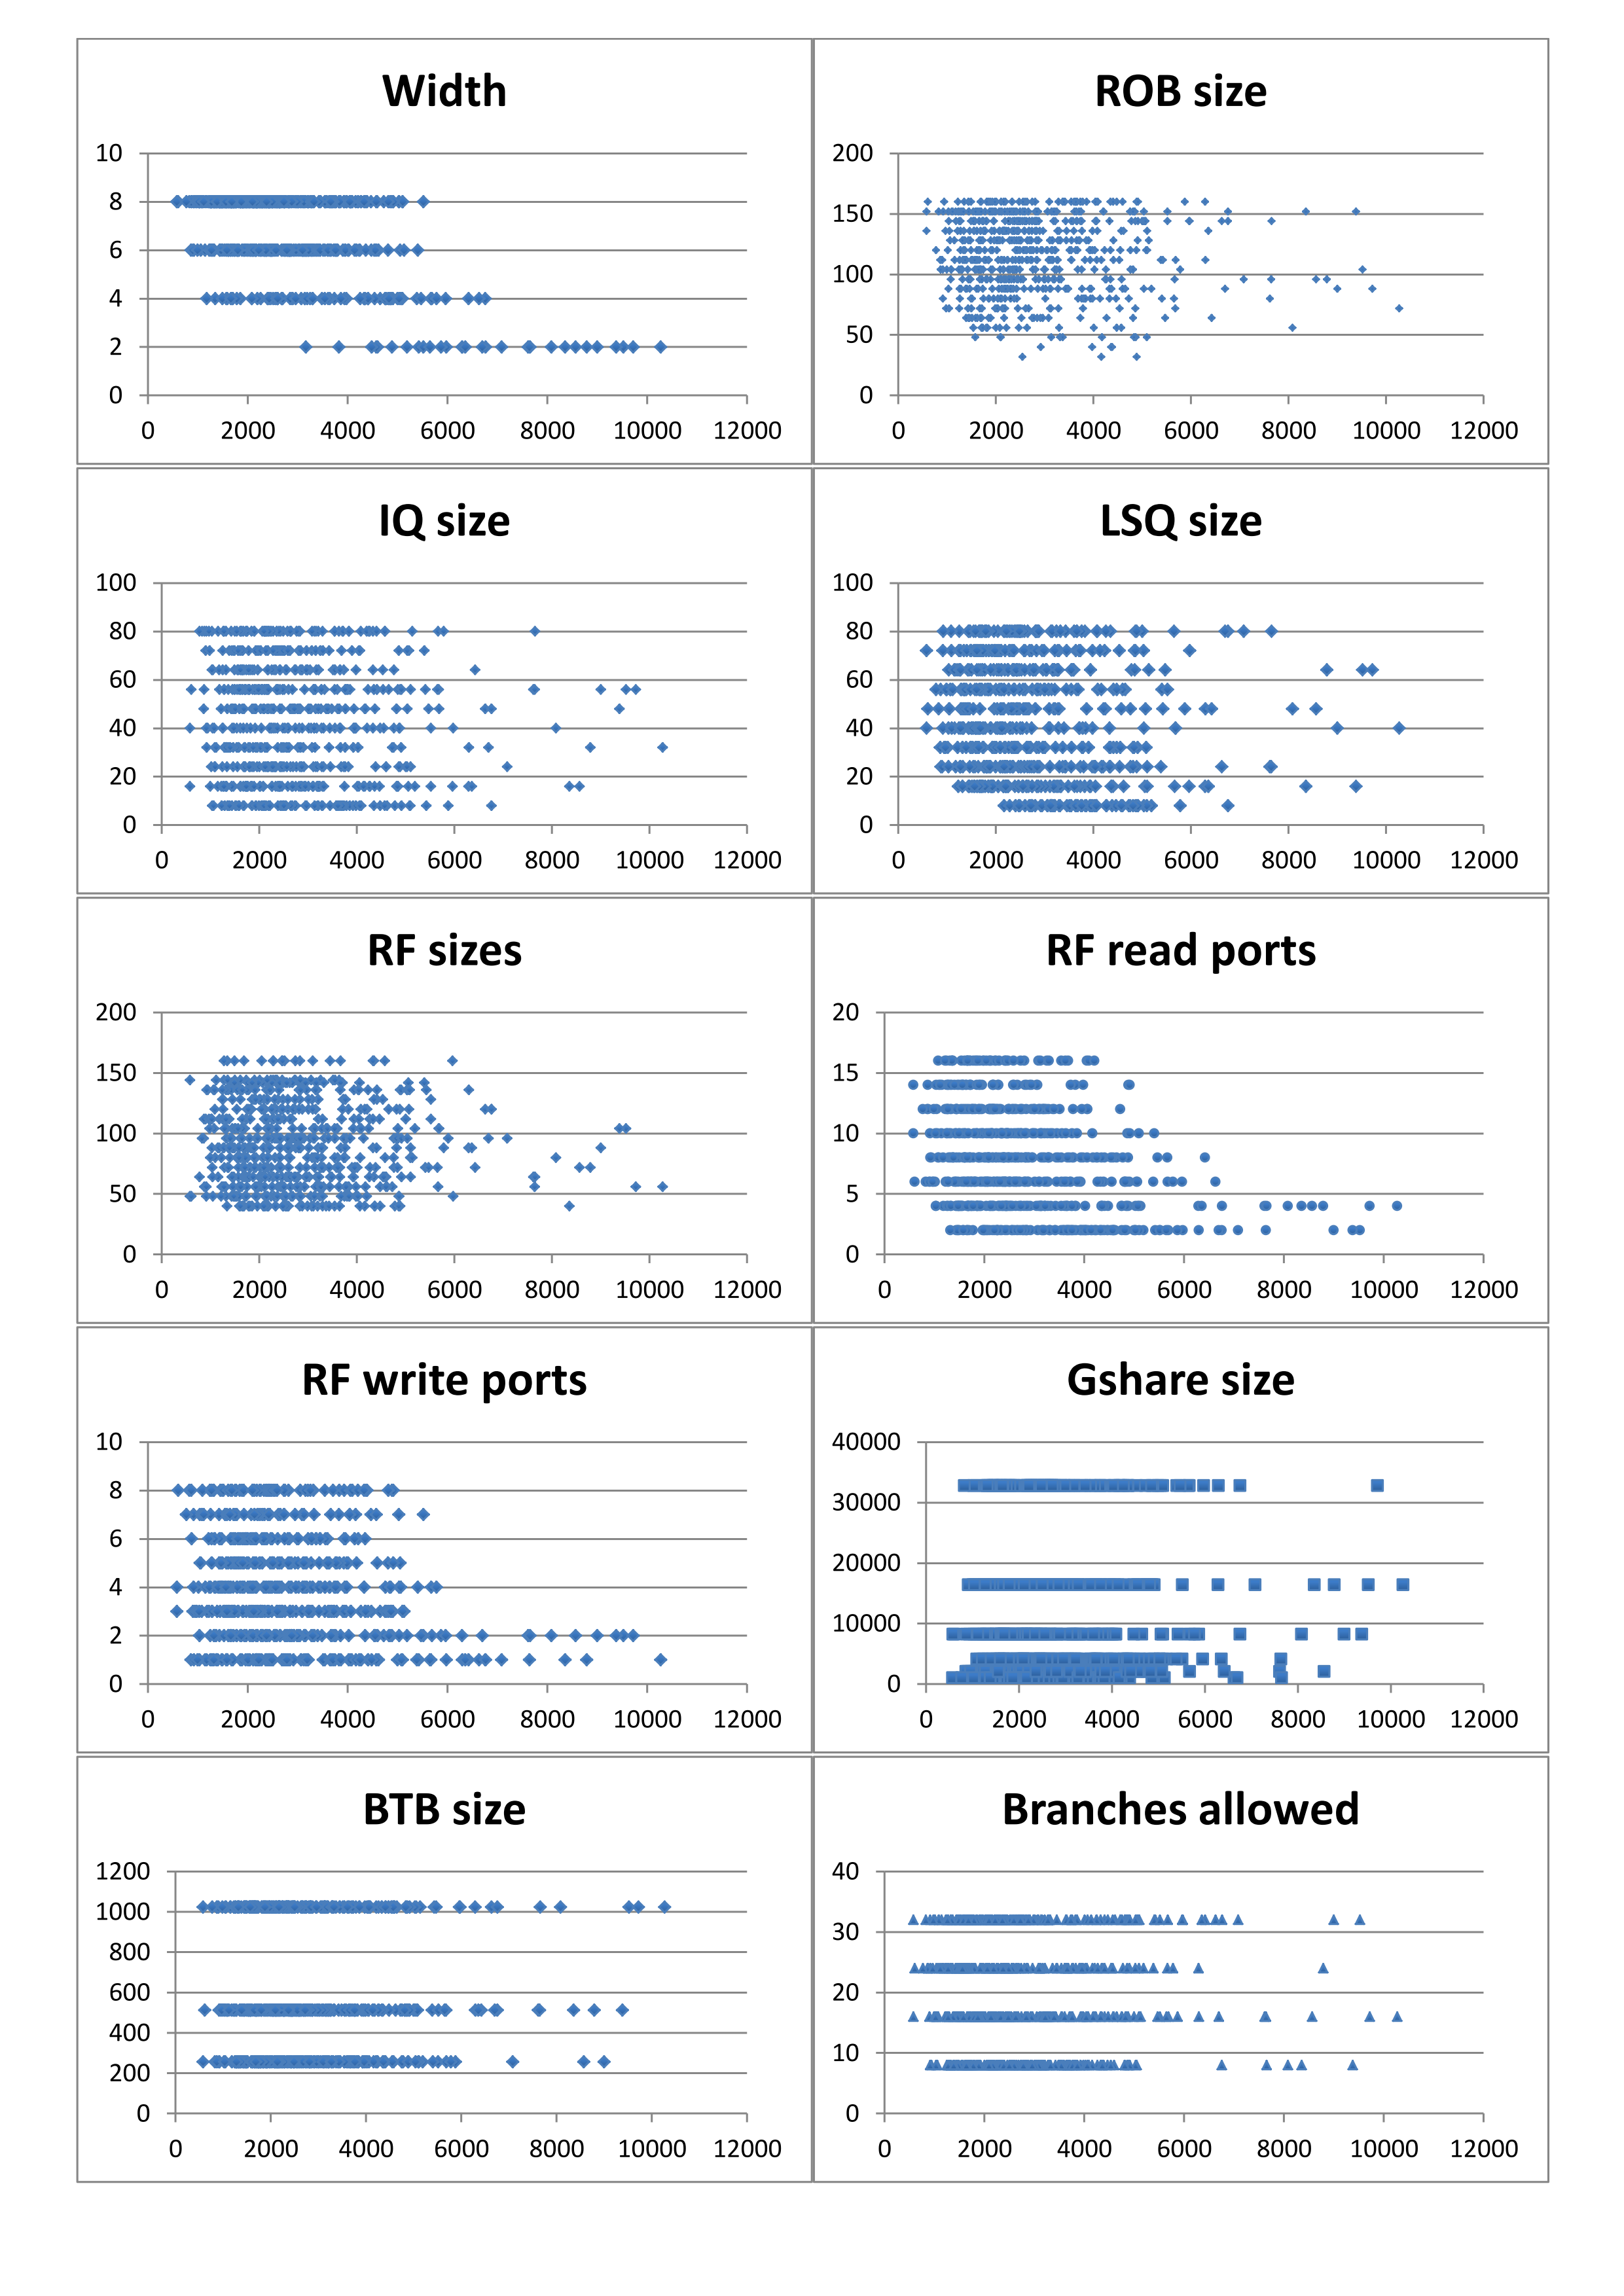
\includegraphics[height=0.8\textheight]{graph.png}

\end{document}
